\documentclass{beamer}
\usetheme{Warsaw}

\usepackage[utf8]{inputenc}
\usepackage{fancybox}
\usepackage{multimedia} 
\usepackage{subfig}
\usepackage{amsmath}
\usepackage{hyperref}
\usepackage[all]{xy}
\begin{document}


\title[Angewandte Mathematik] % (optional, only for long titles)
{Angewandte Mathematik
\\
\includegraphics[scale=0.15]{images/cover}
}
\subtitle{}
\author[Dr. Johannes Riesterer] % (optional, for multiple authors)
{Dr.  rer. nat. Johannes Riesterer}

\date[KPT 2004] % (optional)
{}

\subject{Angewandte Mathematik}



\frame{\titlepage}

\begin{frame}
    \frametitle{Angewandte Mathematik}
\framesubtitle{Differential}
    \begin{block}{Eigenschaften des Differentials}
Für das Differential einer differenzierbaren Funktion  $f: U \to \mathbb{R}$ gilt für alle $a \in U$:
\begin{itemize}
\item  $df(a) (h) :=  df(a) \cdot h$ ist eine lineare Abbildung von $\mathbb{R}^n$ nach $\mathbb{R}$.
\item $df(a)  \cdot h = \partial_h f(a)$. 
\item $d (f \cdot g) = g(a) d(f) + f(a) dg$
\item $d(f + g) = df + dg$
\end{itemize}
\end{block}
 \end{frame}

\begin{frame}
    \frametitle{Angewandte Mathematik}
\framesubtitle{Differential}
    \begin{block}{Beweis}
\begin{itemize}
\item  Multiplikation mit einer Matrix ist eine lineare Abbildung.
\item Für die Basisvektoren ist per Definition $df(a)  \cdot e_i = \partial_{e_i} f(a)$. Da jeder Vektor $h$ eine Linearkombination der Basisvektoren ist und $df$ linear ist, folgt die Behauptung.
\item Folgt direkt aus der entsprechenden Eigenschaft reeller Funktionen.
\item Folgt direkt aus der entsprechenden Eigenschaft reeller Funktionen.
\end{itemize}
\end{block}
 \end{frame}



\begin{frame}
    \frametitle{Angewandte Mathematik}
\framesubtitle{Lokale Linearisierung}
    \begin{block}{Lokale Linearisierung}
Ist  $f: U \to \mathbb{R}$ differenzierbar, dann gilt für alle $a \in U$ und $h \in \mathbb{R}$ 
\begin{align*}
f(a + h)  =  f(a)  +  df(a) \cdot h + R(h) 
\end{align*}
mit   $\lim_{h \to 0} \frac{R(h)}{ ||h||} = 0$.
\end{block}
    \begin{block}{Bedeutung}
Eine differenzierbare Funktion kann  auf hinreichend kleinen Umgebungen 
beliebig genau durch eine lineare Funktion approximiert werden. 
\end{block}
 \end{frame}

\begin{frame}
    \frametitle{Angewandte Mathematik}
\framesubtitle{Lokale Linearisierung}
    \begin{block}{Beweis}
\begin{figure}[H]
      \centering
    \includegraphics[width=0.4\textwidth]{images/kantenzug}
      \caption{Kantenzug mit achesenparallelen Kanten}
\end{figure}

\end{block}
    \begin{block}{Beweis}

\begin{align*}
& a_0 := a \\
& a_i  := a_{i-1} + h_i e_i;  \;  \;  i = 1, \cdots , n
\end{align*} 
\end{block}

 \end{frame}




\begin{frame}
    \frametitle{Angewandte Mathematik}
\framesubtitle{Lokale Linearisierung}
    \begin{block}{Beweis}
\begin{itemize}
\item $f(a + h) - f(a) = \sum_{i=1}^{n} \bigl( f (a_i)   - f(a_{i-1})   \bigr)$
\pause \item  Mit $\varphi_i(t) : = f(a_i + t e_i)$ gilt  $f(a_i) - f(a_{i-1}) = \varphi_i(h_i)  - \varphi_i(0)$
\pause \item Mittelwertsatz einer Veränderlichen:  Es gibt  $\tau_i$  mit
\begin{align*}
\varphi_i(h_i)  - \varphi_i(0)  = h_i \varphi'(\tau_i) \;.
\end{align*}
\pause \item 
\begin{align*}
f(a + h) - f(a) - df(a) \cdot h = \sum_{i=1}^n  \biggl( \frac{\partial  f(\xi) }{\partial x_i} -    \frac{\partial  f(a) }{\partial x_i}   \biggr) h_i
\end{align*} 
\end {itemize}

 
Da $\varphi'_i(t) = \frac{\partial  f(a_{i-1} + t e_i ) }{\partial x_i}$ und mit $\xi_i: = a_i + \tau_i e_i$ 
\end{block}

 \end{frame}

\begin{frame}
    \frametitle{Angewandte Mathematik}
\framesubtitle{Lokale Linearisierung}
    \begin{block}{Beweis}
\begin{align*}
| f(a + h) - f(a) - df(a) \cdot h |  \leq || h ||_{\infty}  \sum_{i=1}^n  \biggl| \frac{\partial  f(\xi) }{\partial x_i} -    \frac{\partial  f(a) }{\partial x_i}   \biggr | \; . 
\end{align*} 
Für $h \to 0$ gilt $\xi_i \to a$ und da die partiellen Ableitung stetig sind nach Voraussetzung und alle Normen äquivalent sind folgt

\begin{align*}
\lim_{h \to 0} \frac{ f(a + h) - f(a) - df(a) \cdot h}{||h||} = 0 
\end{align*} 

\end{block}

 \end{frame}

\begin{frame}
    \frametitle{Angewandte Mathematik}
\framesubtitle{Lokale Linearisierung}
    \begin{block}{Eindeutigkeit des Differentials}
Umformuliert bedeutet der Satz über die lokale Linearisierung, dass für das Differential einer differenzierbare Funktion
\begin{align}
\lim_{h \to 0} \frac{f(a + h) -f(a) - df(a) h }{||h||} = 0
\end{align}
gilt. Ist $L$ eine weiter lineare Abbildung mit $\lim_{h \to 0} \frac{f(a + h) -f(a) - L(a) h }{||h||}$, so ist $L = df$. Das Differential ist somit eindeutig durch die Eigenschaft der lokalen Linearisierung bestimmt.
\end{block}
 \end{frame}

\begin{frame}
    \frametitle{Angewandte Mathematik}
\framesubtitle{Lokale Linearisierung}
    \begin{block}{Eindeutigkeit des Differentials}
Für $v \in \mathbb{R}^n$ mit $||v|| = 1$ gilt 
\begin {align*}
\bigl( L(a) - df(a) \bigr)(v) & =  \lim_{t \to 0}  \bigl( L(a) - df(a) \bigr) \bigl( \frac{tv}{||tv||} \bigr) \\
& = \lim_{t \to 0} \frac{\bigl( L(a) - df(a) \bigr)(tv) }{||tv||} = 0
\end{align*}
Da jeder Vektor als Linearkombination von Einheitsbasisvektoren dargestellt werden kann, folgt die Behauptung.
\end{block}
 \end{frame}





\begin{frame}
    \frametitle{Angewandte Mathematik}
\framesubtitle{(Baby) Kettenregel}
    \begin{block}{Wege}
Ein Weg ist eine Abbildung  
\begin{align*}
& \gamma:  [a,b] \to \mathbb{R}^n \\
& \gamma (t) :=  \begin{pmatrix} \gamma_1(t) \\ \vdots \\ \gamma_n(t) \end{pmatrix}
\end{align*}
mit reellen, stetigen Funktionen $y_i : [a,b] \to \mathbb{R}$ (Damit ist auch $\gamma$ stetig).
\end{block}

 \end{frame}

\begin{frame}
    \frametitle{Angewandte Mathematik}
\framesubtitle{Baby Kettenregel}
\begin{figure}[H]
      \centering
    \includegraphics[width=0.8\textwidth]{images/EbeneKurve}
      \caption{Quelle: Wikipedia: https://de.wikipedia.org/wiki/Datei:EbeneKurve.png}
\end{figure}

 \end{frame}


\begin{frame}
    \frametitle{Angewandte Mathematik}
\framesubtitle{Baby Kettenregel}
    \begin{block}{Weg}
Ein Weg ist eine Abbildung  
\begin{align*}
& \gamma:  [a,b] \to \mathbb{R}^n \\
& \gamma (t) :=  \begin{pmatrix} \gamma_1(t) \\ \vdots \\ \gamma_n(t) \end{pmatrix}
\end{align*}
mit reellen, stetigen Funktionen $y_i : [a,b] \to \mathbb{R}$ (Damit ist auch $\gamma$ stetig).
\end{block}

 \end{frame}


\begin{frame}
    \frametitle{Angewandte Mathematik}
\framesubtitle{Baby Kettenregel}
    \begin{block}{Differenzierterer Weg}
Der Weg $\gamma$ heißt differenzierbar, falls alle Ableitungen $\gamma_i'(t)$ existieren. In diesem Fall bezeichnen wir
\begin{align*}
 \gamma' (t) :=  \begin{pmatrix} \gamma'_1(t) \\ \vdots \\ \gamma'_n(t) \end{pmatrix}
\end{align*}
\end{block}

 \end{frame}

\begin{frame}
    \frametitle{Angewandte Mathematik}
\framesubtitle{Baby Kettenregel}
    \begin{block}{Baby Kettenregel}
Sei $\gamma: I \to U$ ein differenzierterer Weg und $f: U \to \mathbb{R}$ eine differenziertere Funktion. Dann ist $f \circ \gamma : I \to \mathbb{R}$ differenzierbar und hat die Ableitung
\begin{align*}
\frac{d(f \circ \gamma)}{dt}(t) = df(\gamma(t))\gamma'(t) = \sum_{i=1}^n  \frac{\partial f (\gamma(t))}{\partial x_i} \gamma'_i(t)
\end{align*} 
\end{block}
    \begin{block}{Verkettung}
$(f \circ \gamma)(t) := f (\gamma(t)) $

\end{block}
 \end{frame}


\begin{frame}
    \frametitle{Angewandte Mathematik}
\framesubtitle{Baby Kettenregel}
    \begin{block}{Beweis}
\begin{itemize}
\item $\gamma$ und $f$ differenzierbar
\begin{align*}
& \gamma (t + k) = \gamma(t) + k \gamma'(t) + r_1 (k) |k|\\
& f(\gamma(t) + h) = f(\gamma(t)) + df(\gamma(t)) \cdot \gamma'(t) h +  r_2 (h)  ||h|| 
\end{align*}
 $lim_{k \to 0} r_1(k) = 0$, $lim_{h \to 0} r_2(h) = 0$.
\pause \item  $h:= \gamma(t + k) - \gamma(t)$ 
\begin{align*}
f(\gamma(t + k)) = f(\gamma(t)) + df(\gamma(t)) \cdot \gamma'(t) k +  R(k)
\end{align*}  
mit dem Restglied
\begin{align*}
R(k) := & df(\gamma(t)) r_1(k) |k| + r_2 \bigl( \gamma (t + k) \\
 & - \gamma(t) \bigr) ||\gamma'(t) k + r_1(k) |k| || 
\end{align*}  
\end{itemize}
\end{block}
 \end{frame}

\begin{frame}
    \frametitle{Angewandte Mathematik}
\framesubtitle{Baby Kettenregel}
    \begin{block}{Beweis}
\begin{itemize}
\item $\lim_{k \to 0} R(k) = 0$.
\end{itemize}
\end{block}
 \end{frame}



\begin{frame}
    \frametitle{Angewandte Mathematik}
\framesubtitle{Vertauschen von Ableitungen}
    \begin{block}{Satz von Schwarz}
Wenn Für eine Funktion $f: U \to \mathbb{R}$ die Ableitungen $\frac{\partial}{\partial x_i} f(a)$, $\frac{\partial}{\partial x_j}f(a)$ und $ \frac{\partial}{\partial x_i}\frac{\partial }{\partial x_j} f(a)$ existieren und letztere stetig ist, dann existiert auch $ \frac{\partial}{\partial x_j}\frac{\partial }{\partial x_i} f(a)$ und es gilt
\begin{align*}
\frac{\partial}{\partial x_i}\frac{\partial }{\partial x_j} f(a) = \frac{\partial}{\partial x_j}\frac{\partial }{\partial x_i} f(a)
\end{align*}
\end{block}
    \begin{block}{Bedeutung}
Die Reihenfolge spielt beim wiederholten ableiten keine Rolle.
\end{block}
 \end{frame}



\begin{frame}
    \frametitle{Angewandte Mathematik}
\framesubtitle{Höhere Ableitungen}
    \begin{block}{$\mathcal{C}^k$-Funktionen}
Eine  Funktion  $f: U \to \mathbb{R}$ für die alle partiellen Ableitungen 
\begin{align*}
 \frac{\partial}{\partial x_{i_1}} \cdots   \frac{\partial}{\partial x_{i_k}} f(a)
\end{align*}
mit $i_1 + \cdots + i_k \leq k$ existieren und stetig sind heißt $\mathcal{C}^k$-Funktion oder $k$-mal stetig differenzierbar.
\end{block}
    \begin{block}{$\mathcal{C}^k$-Funktionen}
 Eine  $\mathcal{C}^1$-Funktion ist also eine differenzierbare Funktion.
\end{block}
 \end{frame}


\begin{frame}
    \frametitle{Angewandte Mathematik}
\framesubtitle{Höhere Ableitungen}
    \begin{block}{p-te Ableitung}
Für  eine Funktion  $f: U \to \mathbb{R}$, $a \in U$ und Vektoren $v^1, \cdots , v^p \in \mathbb{R}^n$ heißt 
\begin{align*}
d^pf(a) \bigl(v^1, \cdots , v^p  ) := \partial_{v^1} \hdots \partial_{v^p} f(a)
\end{align*}
die $p$-te Richtungsableitung von $f$. Sie ist wegen dem Satz von Schwarz wohldefiniert.

\end{block}
    \begin{block}{}
\begin{align*}
d^pf(a) \bigl(v^1, \cdots , v^p  ) = \sum_{i_1 = 1}^n \cdots \sum_{i_p = 1}^n  \frac{\partial}{\partial x_{i_1}} \hdots \frac{\partial}{\partial x_{i_p}} f(a) \cdot v^1_{i_1} \cdots v^p_{i_p} \; .
\end{align*}
Für einen Vektor $z \in \mathbb{R}^n$ definieren wir $d^pf(a) z^p := d^pf(a) \underbrace{(z, \cdots , z)}_{p-mal} \;.$

\end{block}
 \end{frame}


\begin{frame}
    \frametitle{Angewandte Mathematik}
\framesubtitle{Höhere Ableitungen}
    \begin{block}{Hessematrix}
Für $p = 2$ und $u,v \in \mathbb{R}^n$ ist
\begin{align*}
d^2f(a) \bigl(u , v ) = \sum_{i = 1}^n \sum_{j = 1}^n \frac{\partial}{\partial x_{i}}  \frac{\partial}{\partial x_{j}} f(a) v_{i}  u_{i} 
\end{align*}
und mit 
\begin{align*}
f''(a) : = \begin{pmatrix}  \frac{\partial}{\partial x_{1}} \frac{\partial}{\partial x_{1}} f(a)   &  \cdots &  \frac{\partial}{\partial x_{1}} \frac{\partial}{\partial x_{n}} f(a) \\
\vdots & & \vdots  \\
 \frac{\partial}{\partial x_{n}} \frac{\partial}{\partial x_{1}} f(a)   &  \cdots &  \frac{\partial}{\partial x_{n}} \frac{\partial}{\partial x_{n}} f(a)
\end{pmatrix} 
\end{align*}
ist $d^2f(a) \bigl(u , v ) = u^T  \cdot f''(a) \cdot v$. Die Matrix $f''(a)$ wird auch Hesse-Matrix genannt. Nach dem Satz von Schwarz ist sie symmetrisch.
\end{block}
 \end{frame}

\begin{frame}
    \frametitle{Angewandte Mathematik}
\framesubtitle{Höhere Ableitungen}
    \begin{block}{Taylorapproximation}
Sei   $f: U \to \mathbb{R}$ eine $\mathcal{C}^{p+1}$-Funktion und $x,a \in U$, so dass die Verbindung zwischen $x$ und $a$ in $U$ liegt.
Dann gilt
\begin{align*}
f(x) = f(a) + \sum_{k=1}^{p} d^k f(a) (x-a)^k + R_{p+1} (x;a)
\end{align*}
mit dem Restglied $R_{p+1} (x;a) := \frac{1}{(p+1)!} d^{p+1}f(\xi) (x-a)^{p+1}$ für ein $\xi \in [a,x]$.

\end{block}
 \end{frame}


\begin{frame}
    \frametitle{Angewandte Mathematik}
\framesubtitle{Höhere Ableitungen}
    \begin{block}{Beweis}
Sei $h := (x-a)$ und $F(t) := f(a + th)$ mit $t \in [0,1]$. Wiederholte Anwendung der (Baby) Kettenregel mit $\gamma(t) := a +th$ ergibt
\begin{align*}
& F'(t) = \sum_{i=1}^n  \frac{\partial}{\partial x_{i}} f(a + th) h_i \\
& F''(t) =\sum_{j=1}^n \sum_{i=1}^n   \frac{\partial}{\partial x_{j}} \frac{\partial}{\partial x_{i}} f(a + th) h_i h_j \\
& \vdots \\
& F^p(t) =  \sum_{i_1=1}^n  \cdots \sum_{i_p=1}^n   \frac{\partial}{\partial x_{i_1}} \cdots \frac{\partial}{\partial x_{i_p}} f(a + th) h_{i_1} \cdots  h_{i_p}  \; .
\end{align*}
\end{block}
 \end{frame}

\begin{frame}
    \frametitle{Angewandte Mathematik}
\framesubtitle{Höhere Ableitungen}
    \begin{block}{Beweis}
Mit der Taylorapproximation für Funktionen einer Veränderlichen folgt
\begin{align*}
 F(1) = F(0) + F'(0) + \frac{1}{2!} F''(0) + \cdots + \frac{1}{p!} F^p(0) + R_{p+1} 
\end{align*}
mit dem Restglied $ R_{p+1}  :=  \frac{1}{(p+1)!}  F^p(\tau)$ mit $\tau \in [0,1]$.
Da nach Konstruktion $F(0) = f(a)$ und $F(1)= f(x)$ folgt insgesamt die Behauptung.
\end{block}
 \end{frame}

\begin{frame}
    \frametitle{Angewandte Mathematik}
\framesubtitle{Höhere Ableitungen}
    \begin{block}{Taylorapproximation}
Sei $T_p(x,a) =  f(a) + \sum_{k=1}^{p} d^k f(a) (x-a)^k$ die Taylorraproximation einer $\mathcal{C}^{p}$-Funktion. Dann gilt: 
\begin{align*}
\lim_{x \to a} \frac{f(x) - T_p(x;a)}{  || x-a  ||^p} = 0 \;. 
\end{align*}
\end{block}

    \begin{block}{Bedeutung}
Die Taylorapproximation vom Grad $p$ konvergiert polynominell vom Grad $p$ gegen $0$.
\end{block}
 \end{frame}

\begin{frame}
    \frametitle{Angewandte Mathematik}
\framesubtitle{Höhere Ableitungen}
    \begin{block}{Beweis}
Da die partiellen Ableitungen stetig sind, gibt es für jedes $\epsilon > 0$ ein Radius $r >0$, dass für alle $y \in K_r(a)$
\begin{align*}
\frac{1}{p!} (d^pf(y) -d^pf(a))h^p \leq \epsilon ||h||_{\infty}^p \; . 
\end{align*}
Mit der Taylorapproximation ist 
\begin{align*}
f(x) = & T_{p-1}(x, a) +  \frac{1}{p!} d^{p}f(\xi) (x-a)^{p} \\
 = & T_p(x,a) +   \frac{1}{p!} \bigl( d^pf(\xi) -d^pf(a) \bigr) h^p (x-a)^p
\end{align*} 
Mit obiger Abschätzung folgt die Behauptung.
\end{block}
 \end{frame}


\begin{frame}
    \frametitle{Angewandte Mathematik}
\framesubtitle{Extrema}
    \begin{block}{Extrema}
Sei $f : X \subset \mathbb{R}^n \to \mathbb{R}$ eine relle Funktion.  Ein Punkt $a \in  X$ heißt lokales Maximum bzw. Minimum, falls eine Umgebung $U$ von $a$ existiert, so dass $f(x) \leq f(a)$ bzw.  $f(x) \geq f(a)$ für alle $x \in U$ gilt. Liegt einer der beiden Fälle vor, so spricht man von einem lokalen Extremum. Gilt strikt $f(x) <  f(a)$ bzw.  $f(x) > f(a)$ , so nennt man das Extremum isoliert. Ist $U = X$ so nennt man es auch globales Maximum bzw. Minimum.
\end{block}
 \end{frame}


\begin{frame}
    \frametitle{Angewandte Mathematik}
\framesubtitle{Extrema}

\begin{figure}[H]
      \centering
    \includegraphics[width=0.8\textwidth]{images/MaximumParaboloid}
      \caption{Quelle: Wikipedia: https://en.wikipedia.org/wiki/File:MaximumParaboloid.png}
   \end{figure}
 \end{frame}

\begin{frame}
    \frametitle{Angewandte Mathematik}
\framesubtitle{Extrema}

\begin{figure}[H]
      \centering
    \includegraphics[width=0.8\textwidth]{images/MaximumCounterexample}
      \caption{Quelle: Wikipedia: https://en.wikipedia.org/wiki/File:MaximumCounterexample.png}
\end{figure}
 \end{frame}



\begin{frame}
    \frametitle{Angewandte Mathematik}
\framesubtitle{Extrema}
    \begin{block}{Extrema}
 Ist $f: U  \to \mathbb{R}$ differenzierbar und hat  $f$ in $a \in U$ ein lokales Extremum, so gilt 
\begin{align*}
\frac{\partial}{\partial x_{1}} f(a) = \cdots  = \frac{\partial}{\partial x_{n}} f(a) = 0 \;.
\end{align*}
Dies ist gleichbedeutend mit $df(a) = 0$.
\end{block}
    \begin{block}{Kritischer Punkt}
 Ein Punkt $a$ mit $df(a) = 0$ wird kritischer Punkt genannt.
\end{block}

 \end{frame}

\begin{frame}
    \frametitle{Angewandte Mathematik}
\framesubtitle{Extrema}
    \begin{block}{Beweis}
Setze $F_k(t) := f(a + t e_k)$. Da $f$ ein Extremum in $a$ hat, hat $F_k$ in einer hinreichend kleinen Umgebung um $0$ ein Extremum. 
Da $F_k$ eine Funktion einer Veränderlichen ist, gilt $F'(0) = 0$. Da $\frac{\partial}{\partial x_k} f(a) = F_k'(0)$ folgt die Behauptung.
\end{block}
 \end{frame}


\begin{frame}
    \frametitle{Angewandte Mathematik}
\framesubtitle{Extrema}
    \begin{block}{Extrema}
 Ist $f: U  \to \mathbb{R}$ eine $\mathcal{C}^2$-Funktion und ist $f'(a) = 0$ für ein $a \in U$. Dann gilt:
\begin{itemize}
\item $f''(a) > 0 \Rightarrow $ $f$ hat in $a$ ein isoliertes lokales Minimum.
\item $f''(a) < 0 \Rightarrow $ $f$ hat in $a$ ein isoliertes lokales Maximum.
\item $f''(a) \gtrless 0 \Rightarrow $ $f$ hat in $a$ einen Sattelpunkt.
\end{itemize} 
\end{block}
 \end{frame}


\begin{frame}
    \frametitle{Angewandte Mathematik}
\framesubtitle{Extrema}
    \begin{block}{Beweis}

Sei $f'(a) = 0$ und $f''(a) > 0$. Mit der Taylorformel gilt für hinreichend kurze Vektoren $h \in \mathbb{R}^n$
\begin{align*}
f(a + h) = f(a) + \frac{1}{2} h^T f''(a) h + R(h)
\end{align*}
mit $\lim_{h \to 0} \frac{R(h)}{ ||h||^2} = 0$. Für $||h|| \leq 1$ hat $ h^T f''(a) h $ sein Maximum $m$ auf dem Einheitskreis $\{ h \in \mathbb{R}^n \; | \; ||h|| = 1 \}$ da $f''(a) > 0$.
\begin{align*}
 h^T f''(a) h  = ||h|| \frac{1}{||h||} h^t  f''(a)  ||h|| \frac{1}{||h||} h \geq m ||h||^2 \;.
\end{align*}
\end{block}
 \end{frame}



\begin{frame}
    \frametitle{Angewandte Mathematik}
\framesubtitle{Extrema}
    \begin{block}{Beweis}
Wir wählen $\epsilon$ so klein, dass $R(h) \leq \frac{m}{2}  ||h||^2$ gilt für $||h|| < \epsilon$  (was geht wegen Taylorformel).
Damit erhalten wir
\begin{align*}
f(a + h) \geq f(a) +  m ||h||^2 \;.
\end{align*}
und damit hat $f$ ein lokales Minimum in $a$.

Der Fall $f''(a) < 0$ wird mit Betrachtung von $-f$ durch den vorigen Fall bewiesen.
\end{block}
 \end{frame}



\begin{frame}
    \frametitle{Angewandte Mathematik}
\framesubtitle{Extrema}
    \begin{block}{Beweis}


Es sei nun $f''(a) \gtrless 0$ und $v$ mit $v^T f''(a) v > 0$ und $w$ mit $w^T f''(a) w > 0$. Betrachten wir die Funktionen
\begin{align*}
F_v (t) := f(a + tv) \\
F_w(t) := f(a +tw)
\end{align*}
dann ist 
\begin{align*}
F_v' (t) = 0; \; F_v''(0) = v^T f''(a) v > 0 \\
F_w' (t) = 0; \; F_w''(0) = w^T f''(a) w < 0 \\
\end{align*}
und somit hat $F_v$ ein isoliertes lokales Maximum und $F_w$ ein isoliertes lokales Minimum und damit $f$ kein lokales Extremum  in  $a$.
\end{block}
 \end{frame}



\end{document}

